% !TeX spellcheck = ru_RU
% !TEX root = vkr.tex

\section{Интеграция pysatl-core и рефакторинг архитектуры}
\label{sec:migration}

Раздел описывает решение задач~2 и~3 постановки: собственные распределения библиотеки заменены распределениями ядра \texttt{pysatl-core}, после чего переработаны конвейер оценивания и модель смеси. Библиотека написана на Python 3.12--3.13 с использованием NumPy и SciPy; ядро подключено в версии 0.1.0a0. Код находится в ветке \texttt{main} репозитория \texttt{pysatl-mpest}\footnote{Репозиторий \texttt{pysatl-mpest} (дата обращения: 27.11.2026). \url{https://github.com/PySATL/pysatl-mpest}}, история разработки --- в ветке \texttt{refactor/rework-arch} репозитория \texttt{rework-pysatl-mpest}\footnote{Репозиторий \texttt{rework-pysatl-mpest} (дата обращения: 27.11.2026). \url{https://github.com/PySATL/rework-pysatl-mpest}}. Описанное состояние проверено на коммите \texttt{0521120}.

\subsection{Замена собственных распределений распределениями ядра}
\label{sec:migration-core}

В прежней версии каждое семейство было собственным классом с изменяемыми параметрами. Параметры обновлялись на месте (\texttt{set\_params\_from\_vector}), фиксация отмечалась флагами \texttt{fix\_param} и \texttt{unfix\_param}, а плотность и градиент реализовывались заново для каждого семейства. Это дублировало вероятностный аппарат ядра и не позволяло использовать его семейства и параметризации. После миграции компонентами смеси являются распределения ядра (\texttt{ParametricFamilyDistribution}), а собственные классы распределений и параметров удалены и сохранены в ветке \texttt{archive/legacy-modules}.

Два промежуточных решения не вошли в итоговую архитектуру. Адаптер \texttt{CoreDistributionAdapter}, появившийся на этапе прототипа, удалён: после перехода на распределения ядра он стал лишним слоем. Отдельный адаптер параметров оптимизации (\texttt{ParametricAdapter}), преобразующий параметризации в плоские массивы, не потребовался, так как проекцию на свободные параметры выполняет метод \texttt{view} ядра.

\subsection{Устройство библиотеки после рефакторинга}
\label{sec:migration-design}

Основные классы показаны на рисунке~\ref{fig:migration-classes}.

\begin{figure}[H]
    \centering
    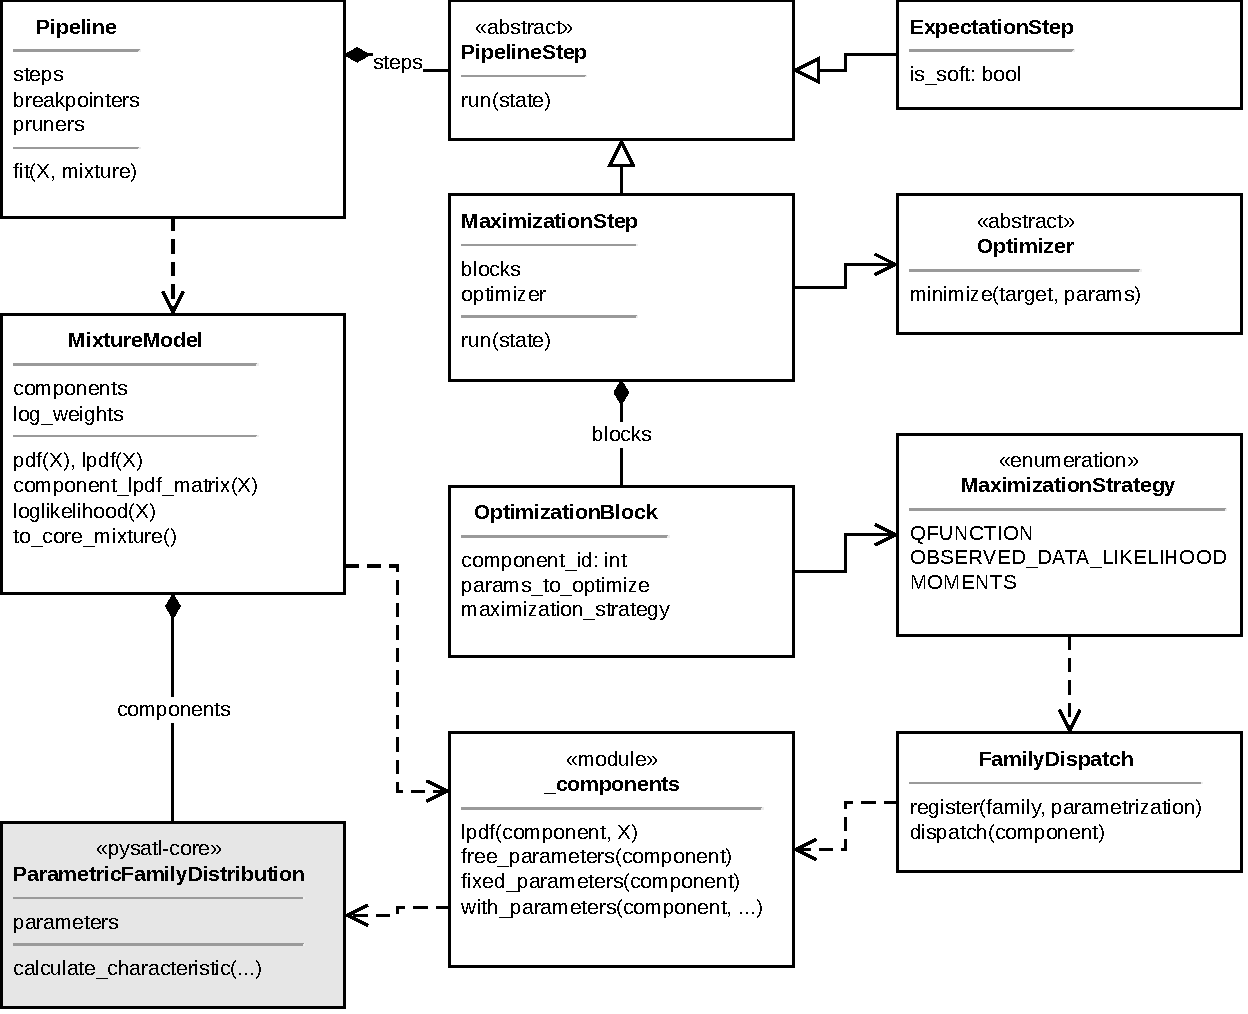
\includegraphics[width=0.95\textwidth]{../figures/migration-classes.pdf}
    \caption{Диаграмма основных классов \texttt{pysatl-mpest} после интеграции \texttt{pysatl-core} и рефакторинга (серым выделены классы ядра)}\label{fig:migration-classes}
\end{figure}

\begin{itemize}
    \item \texttt{MixtureModel} хранит компоненты ядра и логарифмы весов, вычисляет плотность, логарифм плотности и правдоподобие и экспортируется в конечную смесь ядра. Смесь неизменяема: методы \texttt{with\_*} и \texttt{without\_component} возвращают новую смесь;
    \item модуль \texttt{\_components} --- единственное место, где используется внутреннее устройство распределений ядра: вычисление плотности, получение свободных и зафиксированных параметров, построение компонента с новыми значениями параметров. Ядро находится в ранней альфа-версии, поэтому изменение его интерфейса затрагивает только этот модуль. Кроме того, ядро не даёт публичного способа получить частичное семейство из компонента, созданного через \texttt{view}, и доступ к нему изолирован в этом модуле;
    \item \texttt{Pipeline} --- итерационный конвейер: на каждой итерации выполняются шаги (\texttt{ExpectationStep}, \texttt{WeightsStep}, \texttt{MaximizationStep}), затем удаляются компоненты с малым весом и проверяются критерии остановки. \texttt{WeightsStep} обновляет веса по апостериорным весам наблюдений. Оценщики EM, ECM и ECME собирают конвейер из шагов и блоков;
    \item \texttt{MaximizationStep} выполняет блоки \texttt{OptimizationBlock}, в каждом из которых заданы компонент, обновляемые параметры и стратегия \texttt{MaximizationStrategy}: максимизация функции $Q$, максимизация наблюдаемого правдоподобия или метод моментов. Реализацию стратегии выбирает \texttt{FamilyDispatch} по паре <<семейство, параметризация>>.
\end{itemize}

Выбор по паре потребовался, потому что стандартный механизм \texttt{functools.singledispatch} различает реализации по классу первого аргумента, а все компоненты принадлежат одному классу распределения ядра. Для нормального и экспоненциального семейств реализованы аналитические обновления по $Q$, метод моментов реализован только для них, остальные случаи решаются численно оптимизаторами SciPy (метод Нелдера--Мида и метод Пауэлла).

Параметры компонентов ядра неизменяемы, поэтому M-шаг заменяет компонент новым, построенным с обновлёнными значениями. Значения применяются только после успешного выполнения всех блоков. Фиксация подмножества параметров выполняется через \texttt{view}: оптимизируются только свободные параметры, а блок, в котором указан зафиксированный параметр, отклоняется с ошибкой. Стратегия генерации выборок ядра по умолчанию игнорирует начальное состояние генератора, поэтому смесь использует собственную стратегию на основе обратного преобразования, которая учитывает \texttt{random\_state}; это нужно для воспроизводимости экспериментов.

\subsection{Рефакторинг конвейера оценивания}
\label{sec:migration-refactoring}

Переход на ядро сохранил прежнюю схему M-шага и изменяемую смесь; ошибки в них потребовали изменить контракты шагов и смеси.

\textbf{Условная максимизация.} Прежний M-шаг вычислял все блоки по одному снимку смеси и обновлял веса последним. Поэтому условные шаги не видели результатов друг друга и ECM фактически совпадал с EM, а в ECME рост правдоподобия за итерацию не гарантировался. Обновление весов вынесено в шаг \texttt{WeightsStep} перед M-шагом, а блоки M-шага выполняются последовательно: каждый видит результаты предыдущих, независимые блоки объединяются в волны. ECM и ECME принимают упорядоченные группы параметров; ECME выполняет блоки по $Q$ раньше блоков по наблюдаемому правдоподобию, поэтому при мягком E-шаге, без удаления компонентов и с оптимизатором, не ухудшающим целевую функцию, правдоподобие не убывает. Результаты EM не изменились.

\textbf{Неизменяемая смесь.} Хеш смеси вычисляется по её компонентам, а смесь изменялась на месте: смесь-ключ словаря после изменения становилась недоступной, а все записи истории итераций ссылались на один объект и показывали последнюю итерацию. Смесь сделана неизменяемой, как компоненты ядра: каждое изменение возвращает новую смесь. Конвейер перестал копировать смесь, и подгонка ускорилась на 5--49~\% при побитово совпадающих результатах; как и оценки ниже, это значения, полученные в ходе разработки, а не результаты экспериментов.

\textbf{Повторная подгонка.} Критерии остановки и блоки M-шага сохраняли состояние между подгонками, поэтому три подгонки ECM на одних данных давали 33, 18 и 33 итерации, а повторный запуск конвейера после удаления компонента оптимизировал не те компоненты. Теперь состояние сбрасывается в начале каждой подгонки. Кроме того, если веса всех компонентов ниже порога удаления, остаётся компонент с наибольшим весом, а не с наибольшим индексом.

\subsection{Стабилизация и проверка}
\label{sec:migration-check}

Матрица логарифмов плотностей компонент хранится так, что значения одной компоненты расположены в памяти подряд; это ускоряет вычисление суммы по компонентам в E-шаге. По отчёту о задаче\footnote{Отчёт о ходе выполнения задачи 1 (дата обращения: 27.11.2026). \url{https://github.com/iraedeus/diploma-mpest/blob/master/docs/TASK-1-STATUS.md}}, это вернуло скорость E-шага к уровню до перехода: подгонка ECM на двухкомпонентной нормальной смеси выполняется быстрее в 1,5 раза при 2000 наблюдений и в 1,8 раза при 200000. Эти значения получены в ходе разработки и не заменяют экспериментов. Кроме того, исправлены нулевые апостериорные веса для точек вне носителя, нумерация блоков при удалении компонент, учёт только наблюдений из носителя в остановке по правдоподобию и фиксация параметров в шаге по наблюдаемому правдоподобию.

Набор тестов реорганизован по модулям и зависимостям: модульные и интеграционные тесты, вспомогательные функции и заглушки вынесены отдельно. При запуске на коммите \texttt{0521120} 27 ноября 2026 года пройдено 616 тестов, ошибок и пропусков нет, покрытие кода составило 99,78~\% при пороге 80~\%.

Ограничения текущей реализации: используются только безградиентные оптимизаторы без явных границ параметров, градиент логарифма правдоподобия ядра не задействован, модуль прямых оценщиков не содержит реализации, а ядро содержит четыре непрерывных семейства.
